%
%  solutions.tex  2014-12-12  Derrick Kearney created solutions.tex
%
%  Describe how hubcheck is being used to monitor that components of hubs
%  continue to work through software upgrades.
%

% outline:
%
% 1) hubcheck has been deployed to run nightly and weekly tests on hubs
%    the success of hubcheck at alerting us to problems varies.
% 2) introduced 3 new design patterns for building selenium page objects.
% 3) created python modules for interacting with hub tool session containers
%    through SSH/SFTP and some parts of the hub website through Selenium Webdriver.
% 4) can verify correct setup of tool session containers in 1 hour, running 150 tests.
%
% -------------
%

%
% -------------
%
% Summary of results from weekly hubcheck runs:
%
% 1) turbulent hubs
%   -> ccehub
%     * website dashboard web page
%       members_dashboard_my_session_item.test_quick_launch
%       members_dashboard_my_session_storage.test_storage_meter
%     * container packages
%       container_packages.test_wheezy_packages
%     * debian 7 tool session container config
%       container_use_config.test_apps_share64_environ_rappture_link
%       container_use_config.test_apps_share64_environ_rappture_dev_link
%       container_use_config.test_apps_environ_setup_sh_does_not_exist
%       container_icewm_config.test_userconfig_icewm_toolbar
%       container_icewm_config.test_userconfig_icewm_theme
%       container_icewm_config.test_userconfig_icewm_preferences
%       container_icewm_config.test_userconfig_icewm_menu
%       container_icewm_config.test_userconfig_icewm_keys
%       container_config.test_paths_startxvnc
%       container_config.test_paths_pixelflip
%       container_config.test_paths_mergeauth
%       container_config.test_paths_clientaction
%
% 2) new hubs being brought online
%   -> mygeohub
%     * tty problem
%       TestRegisteredUser2.test_tty_recycle
%     * submit, pegasus missing
%       TestContainerSubmitParameterExamples.test_submit_parameter_error_code
%       TestContainerSubmitParameterExamples.test_submit_parameter_glob_file_search
%       TestContainerSubmitParameterExamples.test_submit_parameter_substitute_in_command_arguments
%       TestContainerSubmitParameterExamples.test_submit_change_separator
%       TestContainerSubmitParameterExamples.test_submit_read_csv_params_load_extras_from_file
%       TestContainerSubmitParameterExamples.test_submit_read_csv_params_load_extras_from_args
%       TestContainerSubmitParameterExamples.test_submit_read_params_from_csv_file
%       TestContainerSubmitParameterExamples.test_submit_read_params_file_load_extra_params
%       TestContainerSubmitParameterExamples.test_submit_read_parameters_from_file
%       TestContainerSubmitParameterExamples.test_submit_multiple_parameter_substitution
%       TestContainerSubmitParameterExamples.test_submit_single_parameter_substitution
%     * debian 7 container config
%       container_use_config.test_apps_share_environ_is_directory
%       container_use_config.test_apps_share64_environ_is_directory
%     * container packages
%       container_packages.test_wheezy_packages
%     * website tool session webpage (is there a ticket for this, mygeohub_weekly_20140519024000.log)
%       members_dashboard_my_session_item.test_resume_click
%
% 3) old hubs being upgraded
%   -> pharmahub
%     * submit not working, pegasus missing
%       container_submit_parameter_examples.test_submit_read_params_from_csv_file
%       container_submit_parameter_examples.test_submit_read_params_file_load_extra_params
%       container_submit_parameter_examples.test_submit_read_parameters_from_file
%       container_submit_parameter_examples.test_submit_read_csv_params_load_extras_from_file
%       container_submit_parameter_examples.test_submit_read_csv_params_load_extras_from_args
%       container_submit_parameter_examples.test_submit_parameter_substitute_in_command_arguments
%       container_submit_parameter_examples.test_submit_parameter_glob_file_search
%       container_submit_parameter_examples.test_submit_parameter_error_code
%       container_submit_parameter_examples.test_submit_multiple_parameter_substitution
%       container_submit_parameter_examples.test_submit_change_separator
%     * missing packages:
%       container_packages.test_wheezy_packages
%     * debian 7 tool session container configuration
%       container_use_config.test_apps_share64_environ_rappture_link
%       container_use_config.test_apps_share64_environ_rappture_dev_link
%       container_use_config.test_apps_environ_setup_sh_does_not_exist
%       container_use_config.test_apps_environ_setup_csh_does_not_exist
%       container_config.test_paths_startxvnc
%       container_config.test_paths_pixelflip
%       container_config.test_paths_mergeauth
%       container_config.test_paths_importfile
%       container_config.test_paths_filexfer
%       container_config.test_paths_exportfile
%       container_config.test_paths_clientaction
%
% 4) bugs discovered by hubcheck
%   -> molecularhub, habricentral
%     * side effect of https://hubzero.org/support/ticket/5254 (molecularhub)
%                      https://hubzero.org/support/ticket/5255 (habricentral)
%       parameter_passing_invoke_app_tests.test_1_command_no_templates_no_parameters_file
%       parameter_passing_invoke_app_tests.test_1_command_no_templates_with_parameters_file
%       parameter_passing_invoke_app_tests.test_1_template_0_default_run_template_1
%       parameter_passing_invoke_app_tests.test_1_template_1_default_run_default
%       parameter_passing_invoke_app_tests.test_1_template_1_default_run_template
%     * side effect of https://hubzero.org/support/ticket/5317
%       parameter_passing_url_tests.test_launch_tool_blacklisted_path_1
%       parameter_passing_url_tests.test_launch_tool_invalid_path_4
%     * parameter passing not installed on hub?
%       parameter_passing_url_tests.test_launch_tool_file_format_1
%       parameter_passing_url_tests.test_launch_tool_file_format_2
%       parameter_passing_url_tests.test_launch_tool_file_format_3
%       parameter_passing_url_tests.test_launch_tool_file_format_4
%       parameter_passing_url_tests.test_launch_tool_file_format_5
%       parameter_passing_url_tests.test_launch_tool_file_format_6
%       parameter_passing_url_tests.test_launch_tool_home_expansion_1
%       parameter_passing_url_tests.test_launch_tool_named_file_1
%       parameter_passing_url_tests.test_launch_tool_named_file_2
%       parameter_passing_url_tests.test_launch_tool_whitelisted_path_3
%   -> purr
%     * side effect of https://hubzero.org/support/ticket/5284
%       override causing php to fail before rendering
%       the parameter passing tests may have still passed if we didn't use
%       the tool session web page to see if the session started and to
%       find the session id, but the TestToolSessionApp and TestToolSessionShare
%       tests would still have failed.
%       parameter_passing_invoke_app_tests.test_1_template_0_default_run_template_1
%       parameter_passing_invoke_app_tests.test_1_template_1_default_run_default
%       parameter_passing_invoke_app_tests.test_1_template_1_default_run_template
%       parameter_passing_url_tests.test_launch_tool_file_format_1
%       parameter_passing_url_tests.test_launch_tool_file_format_2
%       parameter_passing_url_tests.test_launch_tool_file_format_3
%       parameter_passing_url_tests.test_launch_tool_file_format_4
%       parameter_passing_url_tests.test_launch_tool_file_format_5
%       parameter_passing_url_tests.test_launch_tool_file_format_6
%       parameter_passing_url_tests.test_launch_tool_home_expansion_1
%       parameter_passing_url_tests.test_launch_tool_named_file_1
%       parameter_passing_url_tests.test_launch_tool_named_file_2
%       parameter_passing_url_tests.test_launch_tool_no_parameters_file
%       parameter_passing_url_tests.test_launch_tool_whitelisted_path_3
%       TestToolSessionApp.test_storage_meter
%       TestToolSessionShare.test_share_session_with_1
%       TestToolSessionShare.test_share_session_with_2
%       TestToolSessionShare.test_share_session_with_3
%       TestToolSessionShare.test_share_session_with_6
%       TestToolSessionShare.test_share_session_with_7
%       TestToolSessionShare.test_share_session_with_8
%       TestToolSessionShare.test_disconnect_1
%     * HAR 500 error? trouble launching tool session container
%       parameter_passing_invoke_app_tests.test_1_command_no_templates_no_parameters_file
%       parameter_passing_invoke_app_tests.test_1_command_no_templates_with_parameters_file
%   -> drinet - no parampassing tests, all issues died when hub was shut down:
%       https://hubzero.org/support/ticket/5328


%In 2013 we started running automated tests on a regular basis on the hubs. In
%February 2014, we deployed a Jenkins server to help manage the automated tests
%and make the test results more accessable to the group. Between February 2014
%and November 2014, we were able to track the results of automated tests. Over
%this time period we have been able to use hubcheck to monitor hubs for bugs as
%they receive website and tool session container upgrades. 


\chapter{HUBCHECK AS A SOLUTION}
\label{chap:solution}

In February of 2014, the HUBzero team deployed a Jenkins
\cite{Jenkins:2015:Online} continuous integration server to help manage
automated tests being run by HUBcheck and to make test results more accessible
to members of the team. Since then, automated test results have been tracked
for runs against the weekly and nightly test suites, two of the most frequently run test
suites offered by HUBcheck. Through the use of the weekly and nightly test
suites, the HUBzero team was able to track the health of hubs and resolve
differences in their setup as they receive website and tool session container
upgrades.

The HUBzero team has tracked the long term results of two of HUBcheck's test
suites. The nightly suite contains 11 test cases that focus on tool session
container access and job submission through the \xfprogramname{submit} command. The
weekly suite contains over 150 test cases and dives deeper into the setup and
workings of the tool session container, including some of the most tedious
tasks to check, which involve interaction between the user's website and tool
session container. As their names suggest, the nightly and weekly suites run on
a nightly and weekly basis respectively.

The health of a hub can be categorized as either \textit{Turbulent},
\textit{Upgraded}, or \textit{New}. Below, we look at each categorization and
use the HUBcheck's weekly and nightly test suites to help identify
opportunities for improvement in the roll out, maintenance, and upgrade of hubs.


\section{Turbulent Hubs}
\label{sec:solution_turbulent}
% explain the meaning of the category
% give an idea of how to identify a hub that fits into this category from the plots
% analyze the experience of one hub that is the representative for this category
% tell how hubs are moved out of this category to a better category.
% give recommendations on how to keep hubs from falling into this category.
%

% between 20140201 and 20150201, 73 new tickets were created on the system.  2
% support tickets on ccehub referenced problems with the tool session container
% or parts of the hub that hubcheck tested (47162 and 47163). we might have
% been able to catch something with 47162, have to check logs. 47163 was
% dealing with rappture problem that affected a specific tool. the version of
% rappture on ccehub that was being used was experimental and the new features
% were not being tested. need to also not how long it has been since a new tool
% was introduced to ccehub or how many users used tool session containers?


%On some hubs, the more tests you add, the more problems you find. These are
%referred to as \textit{Turbulent} hubs and are typical of older hubs that
%have reached the end of their funding cycle, like hub A, where a relaxed
%upgrade strategy, lack of testing plan, and poor communication within the team
%resulted in a hub where errors popped up unexpectedly.  Making changes to this
%type of hub is likely to unknowingly break something.


\begin{figure}[ht!]
        \centering
        \begin{subfigure}[b]{0.65\textwidth}
                \centering
                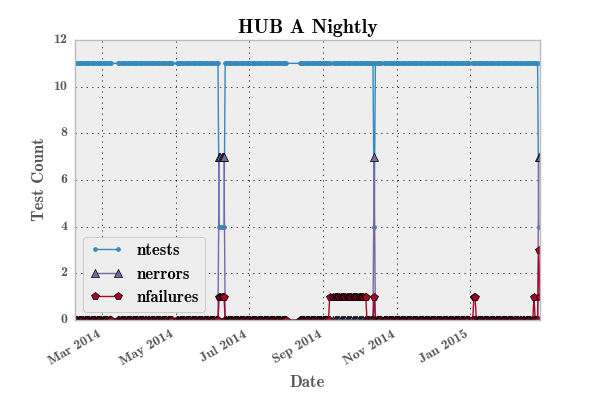
\includegraphics[width=\textwidth]{../../images/summary_plots/hub_a_nightly.png}
        \end{subfigure}
        \begin{subfigure}[b]{0.65\textwidth}
                \centering
                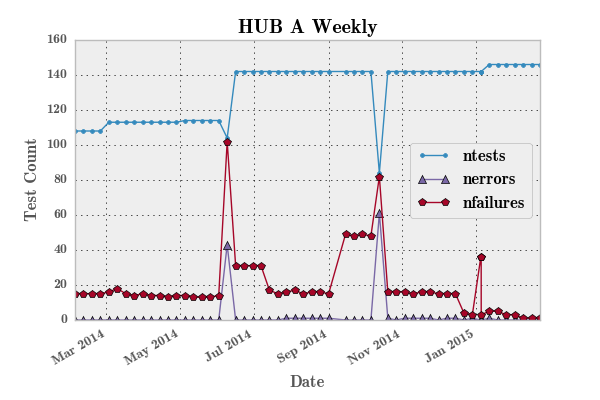
\includegraphics[width=\textwidth]{../../images/summary_plots/hub_a_weekly.png}
        \end{subfigure}
        \caption{ HUBcheck was used to track the health of hub A,
                  a \textit{Turbulent} hub, as website and tool session
                  container software were upgraded through 2014.
                  \textbf{ntests} represents the number of tests in the HUBcheck
                  test suite that ran and completed with either a pass
                  or fail status. \textbf{nerrors} represents the number of
                  HUBcheck tests that partially ran and exited due to
                  an exception being raised. In a small number of cases,
                  the exception is related to an error in the HUBcheck
                  library. An overwhelming amount of the time, these errors
                  signal a problem on the hub that prevented the test
                  from being properly setup. \textbf{nfailures} represents the
                  number of tests that completed and failed due to an
                  assertion.
                  }
        \label{fig:hub_a_health_plots}
\end{figure}


\textit{Turbulent} hubs are typically older hubs that have gone through a
number of software upgrades in the past, when the upgrade process was more
relaxed and testing was less of a priority.  Over the monitoring period, the
HUBcheck test suites were critical in helping the HUBzero team identify and
document problems on hubs as software was upgraded and machines were rebooted.
The history of one particularly turbulent hub, hub A, can be seen in
\Cref{fig:hub_a_health_plots}.

For hub A, tracking began on February 03, 2014 where, at that time, 15 of the
108 tests in the weekly test suite were failing. The testing and failures were
focused on the tool session container configuration. This was an area of active
concern for the team because hub A was in the middle of transitioning the
simulation tools running in containers using the Debian 6 operating system to
containers using the Debian 7 operating system.  Between March 2014 and June
2014, the weekly suite continued to identify 15 test failures.

% hubzero.org ticket \#5286
% hubzero.org ticket \#5317

A number of events occurred on hub A that contributed to its fluctuating
status.  The first manifested itself at the beginning of June 2014 and was
somewhat hidden by another event. The more obvious event at the beginning of
June 2014 shows up as a spike in test failures and errors in the weekly test
suite results. The spike was due to an emergency kernel security patch that
required the shutdown of a machine hosting tool session containers for hub A.
Hidden in the background of this spike was an increase of 17 additional test
failures that were associated with new parameter passing tests that had been
added to the weekly test suite that same week. The newly failing tests showed
that code to support parameter passing was not available on the hub. This is
likely due to the hub needing a website code update.  In the beginning of July
2014, a code update was performed and the next run of the weekly test suite
showed 15 of the 17 previously failing tests began to pass. The two remaining
failing parameter passing tests were identified as bugs in HUBzero's core
implementation and fixes for them are being deployed on various hubs.


% hubzero.org ticket \#6324 (noexec /home)

The second event that elevated test failures occurred at the beginning of
September 2014, when a miscommunication lead to a change in the system that was
not immediately obvious. Symptoms of the problem caused several HUBcheck tests
to fail in the weeks that followed. In the beginning of October 2014, the
problem was identified and fixed.

% hubzero.org ticket \#7079 (noexec /home)

Since October 2014, hub A has shown a decrease in test failures, signaling a
healthier hub. When major events do arise, they have been addressed quickly due
to rigorous monitoring of HUBcheck. For example, early in January 2015,
HUBcheck test failures uncovered a configuration change that occurred after a
system reboot. The HUBzero team was able to quickly identify and resolve the
problem before hub users were affected. With HUBcheck monitoring, hub A is on
its way to becoming like other \textit{Upgraded} hubs.

Turbulent hubs are not common for the HUBzero team. Recently, hubs
that would have been classified as turbulent have been taken down as
opposed to being put through the website code update process. For the
Turbulent hubs that remain in service, HUBcheck's test suites have
been used to monitor their health and work towards applying updates for website
code and tool container configurations.  To keep hubs from falling into this
state, the HUBzero team should continue to add tests to the test suites that
check hub component functionality.



\section{Upgraded Hubs}
\label{sec:solution_upgraded}
% explain the meaning of the category
% give an idea of how to identify a hub that fits into this category from the plots
% analyze the experience of one hub that is the representative for this category
% tell how hubs are moved out of this category to a better category.
% give recommendations on how to keep hubs from falling into this category.

% over the 20140201 - 20150201 monitoring period, pharmahub had 59 support tickets opened.
% 473 - launching tools blank page
% 472 - rappture gui problem with a tool, tool development question
% 459 - explain to user that rappture libraries moved, tool development question
% 458 - tool developement question, june 6 submit error found, problem was fixed in newer versions of submit, problem didn't seem to be related to original question.
% 457 - tool doesnt launch, had previously asked tool developer to update tool, but they didn't. tool development question
% 455 - need debian packages installed, tool development question.
% 453 - tool fails to launch, due to developers not upgrading after hub and container upgrade
% 420 - tools launch with unsigned applet, web issue
% 419 - install new R version, tool development question
% 

Most hubs have a hub health signature that resembles that of an
\textit{Upgraded} hub, where the HUBcheck weekly test suite results start off
with a number of test failures that steadily decrease over time. On
Upgraded hubs, increases in test failures may be seen at predictable
times, such as right after hub updates or during planned maintenance, making them
easy to identify and explain on the nightly and weekly suite result graphs.

\begin{figure}[ht!]
        \centering
        \begin{subfigure}[b]{0.65\textwidth}
                \centering
                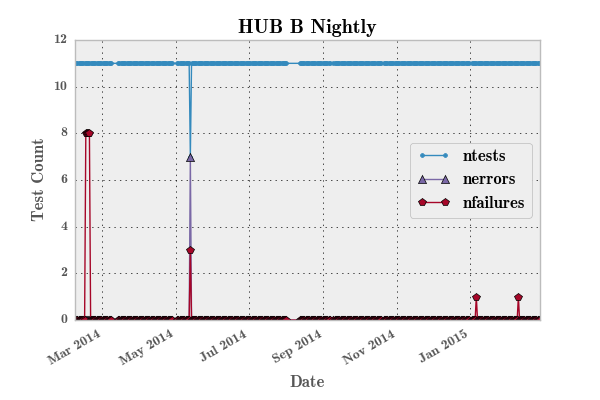
\includegraphics[width=\textwidth]{../../images/summary_plots/hub_b_nightly.png}
        \end{subfigure}
        \begin{subfigure}[b]{0.65\textwidth}
                \centering
                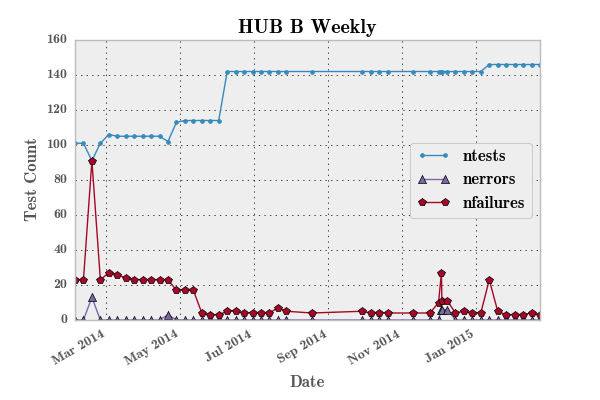
\includegraphics[width=\textwidth]{../../images/summary_plots/hub_b_weekly.png}
        \end{subfigure}
        \caption{ \textit{Upgraded} hubs, like hub B, have a much
                  smoother health graph, where, as time progresses
                  and the number of tests increase, the number of
                  failures decrease. }
        \label{fig:hub_b_health_plots}
\end{figure}

Hub B was brought online at about the same time as hub A. Prior to February
2014, it would have been identified as a \textit{Turbulent} hub due to its use
of vintage website code and tool session container configurations, but today it
is an example of an \textit{Upgraded} hub. The hub received a code update just
before the monitoring period began, but HUBcheck nightly and weekly suites were
still instrumental in helping to identify and fix many of the problems the hub
was experiencing before the upgrade. In February 2014, monitoring of hub B
reported 23 test failures until the end of April. Throughout April, the HUBzero
team focused on reducing test failures on hub B. By the end of April, the
number of failures had dropped from 23 to 17 as new tests were introduced into
the weekly test suite. This decreasing trend is again seen near the middle of
May, when the number of test failures dropped to 4 tests.  The weekly test
suite results graph shows that with the exception of a few false positives, the
number of failures holds steady at 4 tests through the end of November 2014.
In the beginning of December, the software on hub B was upgraded, and HUBcheck
alerted the HUBzero team to a configuration change that caused features on some
web pages to be rendered incorrectly.

The gradually decreasing trend of test failures seen between February and
December 2014 is characteristic of Upgraded hubs. Generally, bugs are
introduced to the system at predictable times such as during system upgrades or
machine reboots. By monitoring test failures through HUBcheck, the HUBzero team
is able to address old problems over time and quickly stamp out new problems.


% not sure what caused the first spike, might have been loosely related to
% hubzero \#4069 (ptys left open after SSH bash shells closed)

% hubzero \#6834 (missing tool session web page decorations after upgrade)

% Jan 12, 2015 - something bad happened to the x virtual frame buffer i think,
% causing false positives to show up for parameter passing tests


\section{New Hubs}
\label{sec:solution_new}
% explain the meaning of the category
% give an idea of how to identify a hub that fits into this category from the plots
% analyze the experience of one hub that is the representative for this category
% tell how hubs are moved out of this category to a better category.
% give recommendations on how to keep hubs from falling into this category.

% datacenterhub - 11/03 spike from switching locators on website without updating hubcheck
% mygeohub - 07/02 spike (hubzero #5511) combining hub data
%          - 11/17 spike fixed by updating hubcheck locators
% polytechhub
% 

\textit{New} hubs are the easiest of hubs to identify. Their nightly and weekly
test suite results start off with nearly zero test failures and over time, new
failures rarely occur. Hubs categorized as New hubs can be reclassified as
Upgraded hubs after they go through a code update cycle. Newly instantiated
hubs managed by the HUBzero team receive a code update on a set schedule of
about every month. This strategy keeps the hubs up to date with bug fixes and
contributes to the reduced number of failures seen in HUBcheck's results.


\begin{figure}[ht!]
        \centering
        \begin{subfigure}[b]{0.65\textwidth}
                \centering
                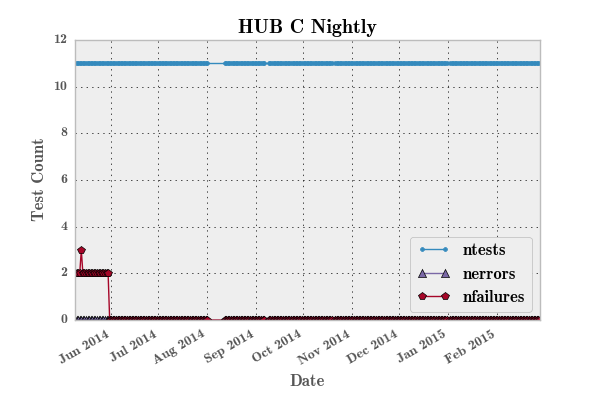
\includegraphics[width=\textwidth]{../../images/summary_plots/hub_c_nightly.png}
        \end{subfigure}
        \begin{subfigure}[b]{0.65\textwidth}
                \centering
                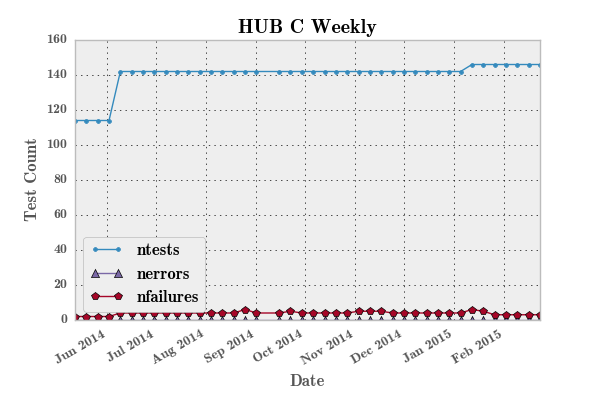
\includegraphics[width=\textwidth]{../../images/summary_plots/hub_c_weekly.png}
        \end{subfigure}
        \caption{For \textit{New} hubs, like hub C, once the setup has completed,
                 the main source of test failures is known problems
                 in the HUBzero's core software.}
        \label{fig:hub_c_health_plots}
\end{figure}


In 2014, the HUBzero team brought up five new hubs.  After the initial setup
was complete, each hub's weekly test suite results showed that the number of
test failures was kept at a steady rate, with nearly all failures being
categorized as known bugs, planned failures, or false positives.

Hub C is was one of the first hubs to be launched in 2014. Since May 2014, hub
C's weekly suite results graph has consistently reported under seven failures.
In June 2014, after additional tests were added to the weekly suite, the number
of test failures rose very slightly due to the identification of known bugs in
the HUBzero software.  Through out September 2014 and November 2014, four false
positives crept up, but for the most part, errors identified by HUBcheck have
stayed very low since the launch of the hub.

New hubs start off with the benefit of being installed with the latest hub code
and configurations. Over time, new features are introduced to the HUBzero
software, bugs are fixed, and the new hubs need to be updated. Consistent
updates and automated tests performed by HUBcheck help keep new hubs working
properly.
